%&bibliografie
\documentclass[presentatie.tex]{subfiles}

\begin{document}

\section{Bibliografie}

\clearrecentlist

% \begin{frame}{Bibliografie}
%     TODO Bibliografie
% \end{frame}

% \begin{saveblock}{code}
% 	\begin{highlightblock}[gobble=8,linewidth=0.5\textwidth,framexleftmargin=0.25em]
%         Code         
% 	\end{highlightblock}
% \end{saveblock}

\lstset{
    alsoletter={$@_!|?$},
}

\updatehighlight{
    name=accentC,
    color=orange,
    add={??}
}

\begin{frame}{Citatiecommando I}
	%We gebruiken dus
	\begingroup

%	\only<2->{\revealcitcmdtrue}
	
	\begin{tabular}{ll}
		\lstinline|as shown in Figure~\\ref\{fig:myPlot\}| & as shown in Figure~1\\
		\lstinline|as shown in \\figref\{fig:myPlot\}| & as shown in Figure~1\\
		\lstinline|as shown in \\autoref\{fig:myPlot\}| & as shown in Figure~1\\
		\lstinline|for this, we use \\eqref\{eq:itsequal\}| & for this, we use (1)\\
		\lstinline|for this, we use \\autoref\{eq:itsequal\}| & for this, we use Equation~1\\
		%\lstinline|this result is well-established ??.| & this result is well-established [1].
		\ifishandout
			\lstinline|is well-established \\cite\{mysource\}.|%
		\else
			\only<1>{\lstinline|is well-established ??.|}\only<2>{\lstinline|is well-established \\cite\{mysource\}.|}% 
		\fi
		%\only<1>{\lstinline|is well-established ??.|}\only<2>{\lstinline|is well-established \\cite\{mysource\}.|} 
%		{\ifrevealcitcmd
%			\lstinline|is well-established \\cite\{mysource\}.|%
%		\else
%			\lstinline|is well-established ??.|%
%		\fi}
		& is well-established [1].
	\end{tabular}
	\endgroup
\end{frame}

\newbox\sizetestbox
\savebox\sizetestbox{\lstinline|\\cite[See chapter 3 of][]\{mysource\}|}

\newlength\columnfakewidth
\setlength\columnfakewidth{\wd\sizetestbox}
%\setlength\columnfakewidth{\dimexpr\columnfakewidth + 1em\relax}

%\newcommand\firstpart[1]{\atleastwidth[5cm]{#1}}
\newcommand\firstpart[1]{\atleastwidth[\columnfakewidth]{#1}}


\begin{frame}[<+->]{Citatiecommando II}
	Variaties in gebruik:
	
	%	\begin{tabular}{ll}
	%		\lstinline|\\cite\{mysource\}|&[1]\\
	%		\only<2->{\lstinline|\\cite[21]\{mysource\}|&[1, p. 21]\\}
	%		\only<3->{\lstinline|\\cite[21--30,8]\{mysource\}|& [1, pp. 21--30, 8]\\}
	%		\only<4->{\lstinline|\\cite[See][21--30,8]\{mysource\}|& [See 1, pp. 21--30, 8]\\}
	%		\only<5->{\lstinline|\\cite[See chapter 3 of][]\{mysource\}|& [See chapter 3 of 1]\\}
	%		\only<6->{\lstinline|\\cite[See chapter 3 of]\{mysource\}|& [1, See chapter 3 of]\\}
	%		\phantom{\lstinline|\\cite[See chapter 3 of]\{mysource\}|}&\phantom{[1, See chapter 3 of]}
	%	\end{tabular}
	\begin{itemize}
		\item \firstpart{\lstinline|\\cite\{mysource\}|}  [1]
		\item \firstpart{\lstinline|\\cite[21]\{mysource\}|}  [1, p. 21]
		\item \firstpart{\lstinline|\\cite[21--30,8]\{mysource\}|}  [1, pp. 21--30, 8]
		\item \firstpart{\lstinline|\\cite[See][21--30,8]\{mysource\}|}  [See 1, pp. 21--30, 8]
		\item \firstpart{\lstinline|\\cite[See chapter 3 of][]\{mysource\}|}  [See chapter 3 of 1]
		\item \firstpart{\lstinline|\\cite[See chapter 3 of]\{mysource\}|}  [1, See chapter 3 of]
		\item \firstpart{\lstinline|\\cites\{mysource\}\{othsource\}|}  [1, 7]
	\end{itemize}
	
\end{frame}

\begin{frame}{Referentielijst items I}
	En hoe verschijnt de eigenlijke referentie dan in \LaTeX?
	
	\begin{center}
		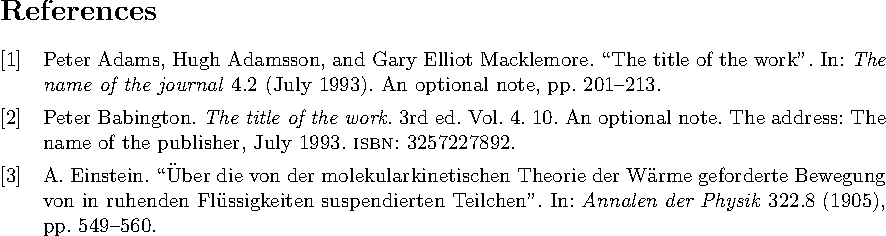
\includegraphics[width=0.9\textwidth]{assets/6_Bibliografie/snippetReferences/snippetReferences.pdf}
	\end{center}
	
	Net zoals \hll|\\tableofcontents| moet je dit expliciet in je bestand plaatsen, maar nu met
	\hll|\\printbibliography|.
\end{frame}


\updatehighlight{
    name=accentB,
    add={@book,@article}
}

\begin{saveblock}{codebox}
	\begin{highlightblock}[linewidth=0.55\textwidth]
		@book{babington,
			author = {Peter Babington},
			title = {Some work},
			publisher = {Publisher},
			year = 1993,
			volume = 4,
			series = 10,
			address = {The address},
			edition = 3,
			month = 7,
			note = {An optional note},
			isbn = {3257227892}
		}
	\end{highlightblock}
\end{saveblock}

\begin{saveblock}{codeboxB}
	\begin{highlightblock}[linewidth=0.55\textwidth]
		@article{adams,
			author  = {Peter Adams
				and Hugh Adamsson},
			title   = {Title},
			journal = {Journal},
			year    = 1993,
			number  = 2,
			pages   = {201-213},
			month   = 7,
			note    = {My note}, 
			volume  = 4
		}
	\end{highlightblock}
\end{saveblock}

\begin{frame}{Referentielijst items II}
	Een item ziet er zo uit:
	
	\begin{columns}
		\begin{column}{0.55\textwidth}
			\useblock{codebox}
		\end{column}
		\begin{column}{0.35\textwidth}%
			\lstinline|\\cite\{babington\}|: [1]
			
			\lstinline|\\fullcite\{babington\}|:\\
			\fullcite{babington}
		\end{column}
	\end{columns}
\end{frame}

%\section{Bib: Configuratie}

\begin{saveblock}{codebox}
	\begin{highlightblock}
		\usepackage[backend=biber]{biblatex}
	\end{highlightblock}
\end{saveblock}

\begin{saveblock}{codeboxB}
	\begin{highlightblock}
		% !BIB TS-program = biber
	\end{highlightblock}
\end{saveblock}

\begin{frame}{Configuratie}
	\useblock{codebox}

	\bigskip

	Op ge\"installeerde versies meer configuratie nodig. Zie extra documentatie.

\end{frame}

% \begin{frame}{Configuratie}
% 	De bibliografie wordt geregeld door het package \hll|biblatex|:
% 	%\par\medskip
% 	\useblock{codebox}
% 	%\par\medskip
% 	... samen met backend Biber.
	
% 	\pause

% 	\bigskip

% 	Archa\"isch systeem: Natbib met backend Bibtex. Niet compatibel.

% 	\begin{center}
% 		{\Large\textbf{Biber expliciet kiezen!}}
% 	\end{center}
	
% 	% \begin{alertblock}{Biber expliciet kiezen}		
% 	% 	\adjustbox{width=\linewidth}{Maar: TeXstudio gebruikt Bibtex als standaard! (ook met \hll|backend=biber|)}
		
% 	% 	\only<3->{Provisionele oplossing: magic comments:
% 	% 		\par\medskip
% 	% 		\useblock{codeboxB}
			
% 	% 		\'Echte oplossing: \hll|Options > Configure TeXstudio > Build > Default Bibliography Tool|, zet op \hll|txs:///biber|.
% 	% 	}
% 	% \end{alertblock}
% 	% }
% \end{frame}

% \begin{frame}{Configuratie}
% 	Archa\"isch systeem: Natbib met backend Bibtex. Niet compatibel.

% 	\begin{alertblock}{Biber expliciet kiezen}		
% 		\adjustbox{width=\linewidth}{Maar: TeXstudio gebruikt Bibtex als standaard! (ook met \hll|backend=biber|)}
		
% 		%\only<1->{
% 		Provisionele oplossing: magic comments:
% 		\par\medskip
% 		\useblock{codeboxB}
		
% 		\'Echte oplossing: \hll|Options > Configure TeXstudio > Build > Default Bibliography Tool|, zet op \hll|txs:///biber|.
% 		%}
% 	\end{alertblock}
% \end{frame}

\begin{saveblock}{codebox}
	\begin{highlightblock}[linewidth=0.4\textwidth]
		% File: bibfile.bib
		@article {...
			...
		}
	
		@book {...
			...
		}
		...
	\end{highlightblock}
\end{saveblock}

\begin{saveblock}{codeboxB}
	\begin{highlightblock}[linewidth=0.6\textwidth]
		% File: document.tex
		\documentclass[a4paper]{article}
		\usepackage{biblatex}
		\addbibresource{bibfile.bib}
		
		\begin{document}
			...
			\printbibliography
		\end{document}
	\end{highlightblock}
\end{saveblock}

\begin{frame}{Overzicht}
	Je hebt dus twee bestanden, die er minimaal zo uitzien.
	
	\bigskip\medskip
	\begin{columns}
		\begin{column}{0.4\textwidth}
			\useblock{codebox}
		\end{column}%
		\begin{column}{0.6\textwidth}
			\useblock{codeboxB}
		\end{column}
	\end{columns}
\end{frame}

\begin{frame}{Stijlen I}
	Bij bibliografie\"en is er een wildernis aan verschillende stijlen:
	
	\begin{itemize}
		\item \hll|numeric|: aa [2], bb [5, 6]\par
		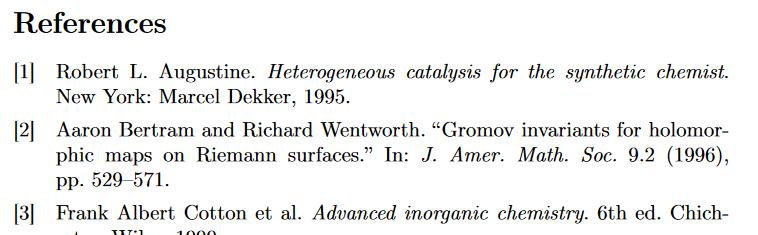
\includegraphics[width=0.8\textwidth]{assets/6_Bibliografie/biblatexStyles/numericReferences.png}
		
		\item\hll|alphabetic|: aa [GMS94], bb [Gon01, Ham97]
		\item\hll|authoryear|: aa John 2003, bb ...
		\item\hll|apa|: aa (Lambert, 1993), bb ...
	\end{itemize}
	In APA: \hll|\\cite| en \hll|\\parencite| verschillen
\end{frame}

\updatehighlight{
	name=accentC,
	add={style=numeric}
}

\begin{saveblock}{codebox}
	%\highlightC{style=numeric}%
	\begin{highlightblock}
		\usepackage[style=numeric]{biblatex}
	\end{highlightblock}
\end{saveblock}

\updatehighlight{
	name=accentC,
	remove={style=numeric}
}

\begin{saveblock}{codeboxD}%
	\begin{highlightblock}
		\DeclareLanguageMapping{english}{english-apa}
	\end{highlightblock}
\end{saveblock}

\begin{frame}{Stijlen II}
	En er zijn nog veel meer stijlen! Voor exacte wetenschappen, gebruiken we gewoon numeric. Zo
	verander je de stijl:
	\useblock{codebox}
	
	\medskip
	Voor APA-stijl heb je daarnaast nodig:
	\useblock{codeboxD}
\end{frame}

\begin{frame}{Sortering}
	\begin{itemize}
		\item \hll|\\usepackage[sorting=none,...]\{biblatex\}|: \\
		In volgorde van verschijning in je document

		\item \hll|\\usepackage[sorting=nty,...]\{biblatex\}| (default):\\
		Naam, dan titel, dan jaar

		\item \hll|\\usepackage[sorting=nyvt,...]\{biblatex\}|:\\
		Naam, dan jaar, dan volume, dan titel

		\item \hll|\\usepackage[sorting=ydnt,...]\{biblatex\}|:\\
		Jaar (\underline{d}escending), dan naam, dan titel

		\item Er zijn er nog meer (zie \hll|biblatex| manual, pagina 47)
	\end{itemize}
\end{frame}

\updatehighlight{
	name=accentC,
	add={and}
}

\begin{saveblock}{codebox}%
	\begin{highlightblock}
		author = {A. Smith and B. Doe and E. Dropper}
	\end{highlightblock}
\end{saveblock}



\begin{frame}{Meerdere auteurs}
	In je \hll|.bib|-bestand, scheid auteurs met \hll|and|:
	\par\medskip\useblock{codebox}
	
	\medskip
	Zo kan \hll|biblatex| controleren hoeveel auteurs het toont.
	\begin{enumerate}
		\item Voor ``... door Peter Adams et al. [1]'' kan je doen met \hll|... door \\textcite\{adams\}|.
		Meer dan \hll|maxnames| [default: 3] (\hll|biblatex| package option) namen, dan
		\hll|minnames| [default: 1] namen.
		\item Voor je bibliografie: meer dan \hll|maxbibnames| [default: \hll|maxnames|], dan
		\hll|minbibnames| [default: \lstinline|minnames|] namen.
	\end{enumerate}

	%Voorbeeld: Peter Adams et al.	
\end{frame}

\updatehighlight{
	name=accentC,
	remove={and}
}

%\begin{lrbox}{\codeboxE}%
%	\highlightC{sorting=none}%
%	\begin{latexlight}
%		\usepackage[sorting=none,...]{biblatex}
%	\end{latexlight}
%\end{lrbox}
%
%\begin{frame}[fragile,allowframebreaks]{Refereren in \LaTeX }
%	%Zo refereer je: \texttt{ \cmd{cite}\{ZelfGekozenLabel1994\} }\\[1.5\baselineskip]
%	Zo refereer je: \lstinline|\cite{ZelfGekozenLabel1994}|\\[1.5\baselineskip]
%	Dit wordt:\\[1.5\baselineskip]
%	\textit{[1]} \qquad \textbf{of} \qquad \textit{(A. Bob, 1994)}, \qquad en er zijn nog meer citeervormen \\[1.5\baselineskip] 
%	
%	Voor deze cursus: referenties tussen blokhaken (dus \textit{[1]})
%	
%	\framebreak
%	
%	Referenties met \texttt{biblatex} and \texttt{biber}:
%	%\begin{latexfigure}
%	%\cmd{usepackage}\texttt{[backend=biber]\{\textcolor{green}{biblatex}\}}
%	%\end{latexfigure}
%	
%	\medskip
%	\usebox\codebox
%	
%	\framebreak
%	Blokhaak-stijl (standaard):
%	%\begin{latexfigure}
%	%    \textbackslash usepackage[\alert{style=numeric-comp}, ...]\{biblatex\}
%	%\end{latexfigure}
%	
%	\medskip
%	\usebox\codeboxB
%	
%	Maakt citaties op deze manier: \\
%	\begin{figure}
%		\textit{Dit is 20\% hoger[1], dan andere auteurs[2, 3]}    
%	\end{figure}
%	
%	\framebreak
%	
%	APA-stijl:
%	\par\medskip
%	\usebox\codeboxC
%	%\begin{latexfigure}
%	%\textbackslash usepackage[\alert{style=apa}, backend=biber]\{biblatex\}
%	%\end{latexfigure}
%	
%	Vereist: 
%	\par\medskip
%	\usebox\codeboxD
%	
%	%\begin{latexfigure}
%	%\textbackslash DeclareLanguageMapping\{english\}\{english-apa\}
%	%\end{latexfigure}
%	
%	Maakt citaties op deze manier: \\
%	\begin{figure}
%		\begin{quote}
%			\textit{Dit is 20\% hoger aldus A (2019), dan andere auteurs (B, 2018; C, 2017)}        
%		\end{quote}
%	\end{figure}
%	
%	Gebruik \lstinline|\parencite| wanneer haken gebruikt moeten worden.
%	
%	\framebreak
%	
%	%\begin{latexfigure}
%	%    \textbackslash usepackage[\alert{sorting=none}, ...]\{biblatex\}\\
%	%\end{latexfigure}
%	
%	\usebox\codeboxE\medskip
%	
%	Zet citaties neer op volgorde waarin ze voorkomen in de tekst.
%\end{frame}

%\begin{lrbox}{\codebox}
%	\begin{latexlight}
%		\usepackage[backend=biber]{biblatex}
%		\addbibresource{bibliografieBestand.bib}
%	\end{latexlight}
%\end{lrbox}
%
%\begin{lrbox}{\codeboxB}
%	\begin{latexlight}
%		\printbibliography
%	\end{latexlight}
%\end{lrbox}

%\section{Bibliography}

%\begin{frame}{Bibliografie I}
%	Zo voeg je een bibliografiebestand in (na \lstinline|\\usepackage|): %(na \texttt{\textbackslash usepackage...}):
%	%\begin{latexfigure}
%	%    \textbackslash usepackage[backend=biber]\{biblatex\}
%	%    \textbackslash addbibresource\{bibliografieBestand.bib\}
%	%\end{latexfigure}
%	
%	\bigskip
%	\usebox\codebox
%	
%\end{frame}
%
%\begin{frame}{Bibliografie II}
%	
%	%\begin{latexfigure}
%	%    \textbackslash printbibliography
%	%\end{latexfigure}
%	\usebox\codeboxB\medskip
%	
%	Geeft een referentielijst met items zoals de volgende:
%	
%	\begin{figure}
%		\centering
%		\includegraphics[width=0.95\textwidth]{assets/citaat}    
%	\end{figure}
%	
%\end{frame}

\updatehighlight{
	name=accentC,
	add={@article}
}

\begin{saveblock}{codebox}%
	\begin{highlightblock}
		@article{Smith1994,
			author = {A. Smith and B. Doe and E. Dropper},
			title = {Titel},
			journal = {Opt. Lett.},
			year = 1994,
			volume = 19,
			number = 11,
			pages = {780-782}
		}
	\end{highlightblock}
\end{saveblock}

\updatehighlight{
	name=accentC,
	add={{ and }}
}

\begin{saveblock}{codeboxB}%
	\begin{highlightblock}
		@article{Smith1994,
			author = {A. Smith and B. Doe and E. Dropper},
			title = {Titel},
			journal = {Opt. Lett.},
			year = 1994,
			volume = 19,
			number = 11,
			pages = {780-782}
		}
	\end{highlightblock}
\end{saveblock}

\updatehighlight{
	name=accentC,
	remove={@article}
}

%\begin{frame}{Bibliografiebestand I}
%	Hoe ziet een bib-bestand eruit?
%	%\begin{center}
%	
%	\bigskip
%	\usebox\codebox\medskip
%	
%	%	\begin{figure}
%	%		\includegraphics[page=1]{assets/verbatim1.pdf}
%	%%\begin{verbatim}
%	%%@article\{\textcolor{red}{Smith1994},\\
%	%%\hspace{1.5em} author = "A. Smith and B. Doe  and E. Dropper",\\
%	%%\hspace{1.5em} title = "Titel",\\
%	%%\hspace{1.5em} journal = "Opt. Lett.",\\
%	%%\hspace{1.5em} year = "1994",\\
%	%%\hspace{1.5em} volume = "19",\\
%	%%\hspace{1.5em} number = "11",\\
%	%%\hspace{1.5em} pages = "780-782"\\
%	%%\}
%	%%\end{verbatim}
%	%	\end{figure}
%	%Dit is een label: \texttt{\textbackslash cite\{Smith1994\}}
%	Dit is een label: \lstinline|\\cite\{Smith1994\}|
%	%\end{center}
%\end{frame}
%
%\begin{frame}{Bibliografiebestand II}
%	Hoe ziet een bib-bestand eruit?
%	%\begin{center}
%	
%	\bigskip
%	\usebox\codeboxB\medskip
%	
%	%\begin{figure}
%	%	%\includegraphics[page=2]{assets/verbatim1.pdf}
%	%
%	%%\begin{verbatim}
%	%%@article\{\textcolor{red}{Smith1994},\\
%	%%\hspace{1.5em} author = "A. Smith \alert{and} B. Doe \alert{and} E. Dropper",\\
%	%%\hspace{1.5em} title = "Titel",\\
%	%%\hspace{1.5em} journal = "Opt. Lett.",\\
%	%%\hspace{1.5em} year = "1994",\\
%	%%\hspace{1.5em} volume = "19",\\
%	%%\hspace{1.5em} number = "11",\\
%	%%\hspace{1.5em} pages = "780-782"\\
%	%%\}
%	%%\end{verbatim}
%	%\end{figure}
%	\begingroup
%	\highlightC{and}%
%	Verschillende auteurs met \lstinline|and| scheiden. 
%	\endgroup
%	%\end{center}
%	
%\end{frame}

\updatehighlight{
	name=accentB,
	add={@article}
}

\begin{saveblock}{codebox}%
	%	\begin{latexlight}
	%		@article{Einstein1905
	%			author = "A. Einstein",
	%			title = "{\"U}ber die von der
	%			molekularkinetischen Theorie der W{\"a}rme
	%			geforderte Bewegung von in ruhenden
	%			Fl{\"u}ssigkeiten suspendierten Teilchen",
	%			journal = "Annalen der Physik",
	%			year = "1905",
	%			volume = "322",
	%			number = "8",
	%			pages = "549-560"
	%		}
	%	\end{latexlight}
	\begin{highlightblock}
		@article{Einstein1905,
			author = {A. Einstein},
			title = {\"Uber die von der
				molekularkinetischen Theorie der W\"arme
				geforderte Bewegung von in ruhenden
				Fl\"ussigkeiten suspendierten Teilchen},
			journal = {Annalen der Physik},
			year = 1905,
			volume = 322,
			number = 8,
			pages = {549-560}
		}
	\end{highlightblock}
\end{saveblock}

% \begin{frame}{Speciale tekens I}
% 	%Hoe ziet een bib-bestand eruit?
% 	%\begin{center}
	
% 	%\bigskip
% 	\useblock{codebox}\medskip
	
% 	%\LaTeX{} in citaties: gebruik \textcolor{red}{"{} "{}} én \textcolor{red}{ \{ \} }
% 	%\end{center}
% \end{frame}

\begin{saveblock}{codebox}%
	\begin{highlightblock}
		@article{Einstein1905,
			author = "A. Einstein",
			title = "{\"U}ber die von der
				molekularkinetischen Theorie der W{\"a}rme
				geforderte Bewegung von in ruhenden
				Fl{\"u}ssigkeiten suspendierten Teilchen",
			journal = "Annalen der Physik",
			year = "1905",
			volume = "322",
			number = "8",
			pages = "549-560"
		}
	\end{highlightblock}
\end{saveblock}

\updatehighlight{
	name=accentB,
	remove={@article}
}

% \begin{frame}{Speciale tekens II}
% 	%Hoe ziet een bib-bestand eruit?
% 	%\begin{center}
	
% 	%\bigskip
% 	\useblock{codebox}\medskip
	
% 	%\LaTeX{} in citaties: gebruik \textcolor{red}{"{} "{}} én \textcolor{red}{ \{ \} }
% 	%\end{center}
% \end{frame}

\begin{saveblock}{codebox}
	\begin{highlightblock}[linewidth=\dimexpr\linewidth - 21.9pt\relax]
		\addcontentsline{toc}{section}{References}
	\end{highlightblock}
\end{saveblock}

\begin{frame}{Opmerkingen}%Goed om te weten I}
	\begin{itemize}
		\item Referentielijst is, net zoals \hll|\\tableofcontents|, niet standaard opgenomen in je
		inhoudstabel. Dit fix je met
		\useblock{codebox}
		
		\item Enkel citaties die je hebt gebruikt verschijnen in je \hll|\\printbibliography|.
		\item Voor bijvoorbeeld experimenten alles uit je \hll|.bib|-bestand in je referentielijst?
		Gebruik \hll|\\nocite\{*\}|, of specifiek item in plaats van ster.
	\end{itemize}
\end{frame}

% \begin{frame}{Goed om te weten II}
% 	\hll|biber| verzorgt een groot deel van de refentielijst, maar wordt niet bij elke compilatie
% 	aangeroepen. Het wordt aangeroepen als	
% 	\begin{itemize}
% 		\item De hulpbestanden (.aux, .bbl, ...) nog genoeg missen.
% 		\item Je in TeXstudio gebruikt \hll|Tools > Bibliography| (F8).
% 		\item Je een nieuwe bron gebruikt in je \hll|.tex|-bestand.
% 		\item TeXstudio ziet dat \hll|.bib|-bestand aangepast is.
% 	\end{itemize}

% 	Maar dus \emph{niet} gewoon omdat je de een paragraaf verwijdert die de laatste citatie van een
% 	referentie had. Doe je zoiets op het laatste moment voor inleveren, compileer, F8, en compileer
% 	nogmaals.
% \end{frame}

\end{document}
